\documentclass[12pt]{article}
\usepackage{setspace}
\linespread{1.2}
\usepackage{fullpage,graphicx,psfrag,amsmath,amsfonts,verbatim}
\usepackage[small,bf]{caption}
\usepackage{amsthm}
% \usepackage[hidelinks]{hyperref}
\usepackage{hyperref}
\usepackage{bbm} % for the indicator function to look good
\usepackage{color}
\usepackage{mathtools}
\usepackage{fancyhdr} % for the header
\usepackage{booktabs} % for regression table display (toprule, midrule, bottomrule)
\usepackage{adjustbox} % for regression table display
\usepackage{threeparttable} % to use table notes
\usepackage{natbib} % for bibliography
\usepackage{tikz}
\usetikzlibrary{arrows.meta}
\input newcommand.tex
\bibliographystyle{apalike}
% \setlength{\parindent}{0pt} % remove the automatic indentation

\title{\textbf{A dynamic model of personality, schooling, and occupational choice}}
\author{Fu Zixuan}
\date{March 2, 2025}

\begin{document}
\maketitle
% \thispagestyle{empty}
% \begin{abstract}

% \end{abstract}

% \newpage
% \thispagestyle{empty}
% \tableofcontents
% \newpage

% \setcounter{page}{1}

\section{Summary}
The paper by \citet{todd2020dynamic} examines the individual's choice of
schooling or working at each period as the optimal solution to maximizing
lifetime utility. This falls under the classical single-agent dynamic problem
with finite periods. The dynamic decision at each period involves the
individual's education and occupation choice. The state that evolves over time
includes an individual's schooling/working experience, which grows over time,
cognitive ability, which is time-invariant, and the novel addition of
individual personality measured in five dimensions, which also develops over
time. While the state is (noisily) observed, the model incorporates an
unobserved element -- latent type, which interacts with the observed state and
the utility functions. By establishing a rich model that includes
cognitive ability, personality traits, and latent type, the authors aim to
answer how personality evolves over time in response to age and experience.

Secondly, although the model restricts the channels through which one variable
affects another, the estimation of model parameters helps quantify the
magnitude of these impacts. For example, the latent type transitions to the
next period type depending on the current type and personality. One can test
whether the latent type is time-variant using the parameter estimates. Lastly,
the model allows the simulation of two different education policies (tuition
reduction and compulsory schooling). While most of the identification results
rely on previous literature, notably \cite{hu2012nonparametric}, the paper
imposes further restrictions as in \citet{hu2017simple} to identify the
probability distribution of CCP, the law of motion of latent type k, and the
law of motion of the observed state. Once the nonparametric identification of
these probabilities is established, the paper uses the simulated methods of
moments to estimate all the model parameters, although the identification
arguments are challenging to establish when using moment-based estimators.

The next section will present the structural model in a simplified way and
briefly mention the estimation steps. Afterwards, I will try to link
the identification arguments in the paper to what we learned in class. While it
seems to me that in the paper, the identification is independent of estimation,
I hope to establish a connection between the two and how one can aid the other.
Lastly, to emphasize the role of unobserved heterogeneity, I will summarize
cases where there is no unobserved heterogeneity (latent type), time-invariant,
and time-variant latent type.

\section{Model}
I simplify the model by abstracting from the specific parametric form of all the functions (utility function, transition probability specification, etc.). I first clarify the key variables and explain how each variable influences one another with some visualization.

\subsection{Variables}
\paragraph{Choice variable} An individual chooses whether to go to school or work in a blue-collar/white-collar job in each period. Since this is a lifetime decision, the choice is a sequence of $d(15), d(16), \ldots, d(49)$ starting from age 15.

\paragraph{Observed state} Among the observed state variables, there are constant ones such as family background $z$ and cognitive ability $c$. \footnote{Even till now, I still do not understand the reason why cognitive ability is set to be time-invariant.} The rest are schooling $g(a)$, working experience $x_1(a), x_2(a)$, and the 5 personality traits $\theta(a)$.

\paragraph{Latent type} The paper adds unobserved heterogeneity to the model because it allows the model to better simulate hypothetical policies as is the case in reality. Here the latent type is denoted by $k(a)$, assuming that the type changes over time. However, the specification of the transition nests time-invariant latent type, which can be tested using the estimate.

\subsection{Dynamics}
The above-mentioned variables can be summarized in the following figure~\ref{fig:viz}.

\begin{figure}[!htbp]
\centering
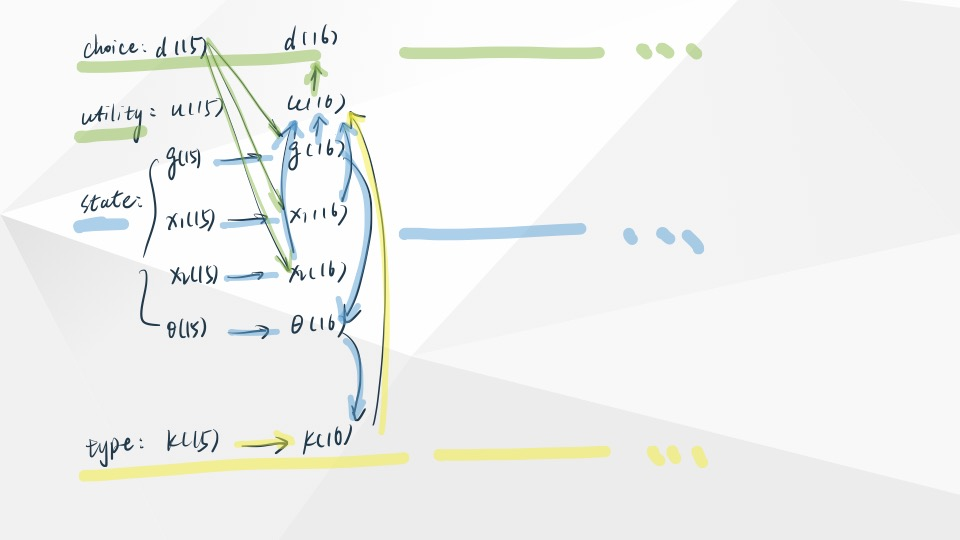
\includegraphics[width=0.6\textwidth]{../Figures/viz.jpg}
\caption{Visualization of the model}
\label{fig:viz}
\end{figure}

\paragraph{Latent type} Going from bottom to top, the current type depends on the previous type via a transition probability matrix. The probability matrix depends on the current personality $\theta(a)$, age $a$, and some shock $\eta(a)$. Therefore, for every transition from $a$ to $a+1$, there is a corresponding transition matrix $L(a)$. This latent type plays a role because it is in the utility function such that, ceteris paribus, current utility from choice $m$, $u_m()$, will be different for different types. This is the only channel through which the type affects the dynamic decision.

\paragraph{Observed state} We now focus on time-changing state variables, personality $\theta(a)$, and experience $g, x_1, x_2$. For personality, the current $\theta(a)$ depends on the very initial $\theta(15)$ as well as age $a$ and years of schooling. This is where model restrictions manifest themselves: only years of schooling can directly affect personality, while working experience does not. It is the paper/author's assumption that later we'll see the education policy that affects years of schooling will impact personality as well. Interestingly, personality is noisily observed in the sense that while the true personality $\theta(a) = f(a, g(a), \theta(a))$ evolves in a deterministic way, the observed personality $\theta^M(a) = \theta(a) + \zeta(a)$ is subject to some measurement error.

For the rest of the variables, evolution is straightforward in the sense that the variable increases if the individual chooses that option $m_0, m_1, m_2$. That is, 
$g(a+1) = g(a) + d_0(a)$, $x_1(a+1) = x_1(a) + d_1(a)$, $x_2(a+1) = x_2(a) + d_2(a)$, where $d_0, d_1, d_2$ are indicator functions of the choice $m_0, m_1, m_2$.

\subsection{(Parametric) Estimation} Now we are ready to establish (restate) the \textbf{single-agent dynamic framework} that has its root in \cite{rust1987optimal}. The choice at each period is obtained by maximizing the lifetime utility. The framework is similar to that of \cite{rust1987optimal}. For example, defining the utility function as $u(\omega, x)$ where $\omega$ is the state variable and $x$ is the choice variable, the value function is
$$V(\omega, \nu) = \max_x u(\omega, x) + \nu(x) + \delta E[V(\omega', \nu')|\omega, x].$$
We can rewrite the value function in terms of the continuation value function such that $V(\omega, \nu) = \max_x \tilde{v}(\omega, x, \nu)$ where $\tilde{v}(\omega, x, \nu) = \tilde{u}(\omega, x) + \nu(x) = u(\omega, x) + \nu(x) + \delta E[V(\omega', \nu')|\omega, x]$. One can establish a clear mapping between the model in the paper and this general framework.

For ease of understanding (for my own purpose), I will rewrite the model in the following way. First, for simplicity, I ignore all shocks except the preference shock $\epsilon(a,s(a), m)$. \footnote{When the agent is making a decision, the personality measurement error $\zeta$ is realized, the latent type transition shock $\eta$ is realized, the wage shock $\xi$ is not realized but the agent takes expectation of it.} Therefore, we have:
\begin{itemize}
    \item The state variable $\omega$ is $(a, s(a))$. The choice variable $x$ is $m$. And $d_m(a)$ is the indicator function of the choice $m$.
    \item The utility function $u(\omega, x)$ is the utility from going to sector $m$, which is $u_m(a, s(a))$.
    \item The continuation value $\tilde{v}(\omega, x, \nu)$ is $\tilde{v}_m(a, s(a),\epsilon)$ where $\tilde{v}_m(a, s(a),\epsilon) = u_m(a, s(a)) + \delta E[V(a+1, s(a+1), \epsilon')|a, s(a), m] + \epsilon(a, s(a), m)$.
    \item The value function $V(\omega, \nu)$ is $V(a, s(a), \epsilon) = \max_m \tilde{v}_m(a, s(a), \epsilon)$.
    \item The conditional choice probability is thus $\Pr(d_m(a) = 1 | a, s(a)) = \frac{\exp(\tilde{u}_m(a, s(a)))}{\sum_{m'} \exp(\tilde{u}_{m'}(a, s(a)))}$.
\end{itemize}
Fixing the parameters, and given a state $(a, s(a))$, we can solve recursively (starting from the terminal period) for the continuation value function $\tilde{v}_m(a, s(a))$ and the conditional choice probability $\Pr(d_m(a) = 1 | a, s(a))$. Second, By simulating the preference shock, one can obtain the choice $m$ at each period. Therefore, taking the simulated choice $m$ at each period, one can compute moments. Lastly, the estimation is then to minimize the distance between the simulated moments and moments from the data.

\subsection{(Nonparametric) Identification}

Up til this point, I haven't linked the the what we have learned from \citet{hu2012nonparametric} to the context of the paper. First, let's recall the set up in \citet{hu2012nonparametric}.
Focusing only on the choice variable $Y_t$ and the latent type $X^*_t$, and take at least 4 periods $Y_1, Y_2,Y_3,Y_4$, their arguments allow us to identify the the distribution of $Y_4|Y_3,X_3^*$ which is the conditional choice probability. In addition, one can identify the transition probability (law of motion of the latent type) $X_4^*|Y_3,X_3^*$. Two main assumptions needed to decompose the matrix $M_{Y_4,y_3,y_2,Y_1}$ is the Markovian property and the limited feedback condition. That is 
\begin{enumerate}
    \item (Markov) Conditional on the current $d(a),s(a),k(a)$, the future $d(a+1),s(a+1),k(a+1)$ is independent of the past $d(a-1),s(a-1),k(a-1)$
    \item (Limited Feedback) Current choice and state $(d(a),s(a))$ only depends on last choice and state $(d(a-1),s(a-1))$ and current type $k(a)$:  $(d(a),s(a))\perp k(a-1)|d(a-1),s(a-1),k(a)$
\end{enumerate}
The second assumption can be graphically represented in figure~\ref{fig:ass}. The assumption is quite weak and can be verified with the structural model. 

\begin{figure}[!htbp]
    \centering
    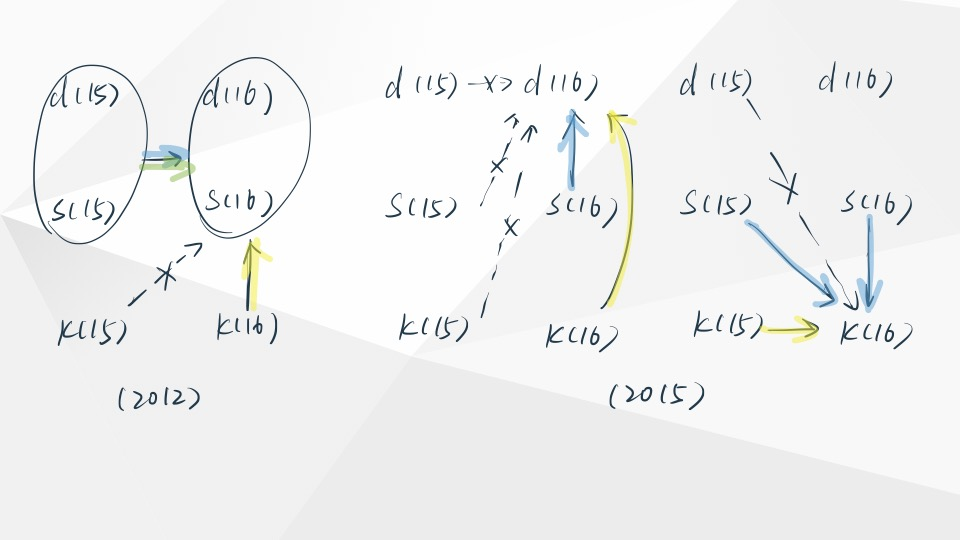
\includegraphics[width=0.6\textwidth]{../Figures/ass.jpg}
    \caption{Limited feedback conditions}
    \label{fig:ass}
    \end{figure}

Moreover, the structural model in the paper imposes more restrction on the feedback condition such that it satisfy an even more restrictive limited feedback condition presented in \citet{hu2017simple}. That is 
\begin{enumerate}
    \item Current choice $d(a)$ only depends on current state $s(a)$ and type $k(a)$: $\Pr(d(a)|s(a),k(a),d(a-1),s(a-1),k(a-1))=\Pr(d(a)|s(a),k(a))$
    \item Current type $k(a)$ only depends on last type $k(a-1)$, current state $s(a)$ and last state $s(a-1)$: $\Pr(k(a)|s(a),s(a-1),k(a-1),d(a-1))=\Pr(k(a)|s(a),s(a-1),k(a-1))$
\end{enumerate}
They can be graphically represented in figure~\ref{fig:ass} as well, which is clearly more restrictive than and nested in the \citet{hu2012nonparametric} assumptions. Under this setting, we can identify $Y_3|X_2^*$ requiring only 3 periods of observations.  In fact, this is almost the same as \citet{hu2008identification}. To see this, let's label choice $Y$, state $M$ and latent type $X^*$
\begin{enumerate}
    \item Step 1: first decompose the probability into three components
$f(Y_2, M_2 \mid M_1, Y_1) = \sum_{x_2^*} f(Y_3 \mid M_3,M_2, x_2^*) f(M_3 Y_2 \mid m_2, x_2^*) f(x_2^* \mid M_2, Y_1)$
\item Step 2: based on the above, we can decompose two matrices
$P(Y_3, m_3 ,y_2 \mid m_2, Y_1) = P(Y_3 \mid m_3, m_2, X_2^*) D_1 (P(y_2 \mid m_3, m_2, X_2^*))D_2(P(m_3\mid m_2,X_2^*))P(X_2^*|m_2,Y_1)$ and 
$P(Y_3, m_3\mid m_2, Y_1) = P(Y_3 \mid m_3, m_2, X_2^*) D_2(P(m_3\mid m_2,X_2^*))P(X_2^*|m_2,Y_1)$
\end{enumerate}
Taking the inverse of second matrix, we can recover the conditional choice probability $P(Y_3 \mid m_3, m_2, x_2^*)$ and the transition probability $P(X_2^*|m_2,Y_1)$. 

\section{Discussion}
As pointed out during the lecture on \citet{postel2002equilibrium}, the specialized structure of the model also satisfies the assumptions of the dynamic model in \citet{bonhomme2019distributional}. Therefore, one can use the latter to test whether the more specialized structural model holds (i.e., whether the specialized assumptions are valid).

In this paper, the interaction seems to work in the opposite direction. The structural model produces estimates that allow us to test whether the latent type is evolving or static, thus facilitating the choice of arguments to prove nonparametric identification. However, even though it is theoretically possible to estimate the conditional choice probability (CCP) using \citet{hu2017simple}, it is empirically difficult due to the large state space \( (a, s(a)) \).

\paragraph{Work Undone} I have not fully understood the rationale behind the implicit ordering of the latent type, both in \citet{hu2012nonparametric} and \citet{hu2017simple}. While previous work assumed there is a monotonic mapping \( G(f_{Y_{t+1}|y_t,x_t^*}) \) that is monotonic in \( x_t^* \), I will need to read \citet{higgins2024learning} to understand how the labeling issue is addressed under certain assumptions.

Secondly, the personality \( \theta \) is observed with measurement error, which is assumed to be normally distributed in the paper. Are there alternative methods to recover the distribution of \( \theta \)? \footnote{To be discussed. I am not sure I fully understood the suggestion.}


\pagebreak \newpage \bibliography{../References/ref.bib}

\end{document}

